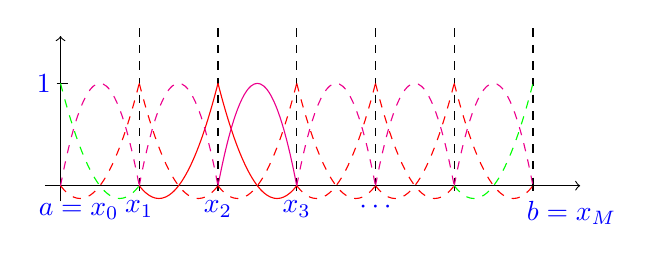
\begin{tikzpicture}
	\draw[->] (-.2,0) -- (6.6,0);
	\draw[->] (0,-.2) -- (0,1.9);		
	
	\draw (-.05,1.3)--(.1,1.3);	
	\foreach \x in {1,2,3,4,5,6}{
		\draw [dashed,thin] (\x,2cm)--(\x,2pt);
		\draw (\x,2pt)--(\x,-2pt);
	}
	\foreach \x/\i in {1/1,2,3/3}
		\node[text=blue,anchor=north] at (\x, -2pt) {$x_\i$};
	
	\node[text=blue,anchor=north] at (4, -2pt) {$\cdots$};
	\node[text=blue,anchor=north west] at (-.4, -3pt) {$a=x_0$};
	\node[text=blue,anchor=north west] at (5.8, -2pt) {$b=x_M$};
	\node[text=blue,anchor=east] at (0,1.3) {1};
	
	\draw[domain=0:1,smooth,variable=\x,xshift=1cm,red] 
		plot ({\x},{1.3*\x*(2*\x-1)});
	\draw[domain=0:1,smooth,variable=\x,xshift=2cm,red] 
		plot ({\x},{1.3*(\x-1)*(2*\x-1)});	
	\draw[domain=0:1,smooth,variable=\x,xshift=2cm,magenta] 
		plot ({\x},{1.3*4*\x*(1-\x)});
	
	\foreach \i/\j in {0/1,2/3,3/4,4/5} {
		\draw[domain=0:1,smooth,variable=\x,xshift=\i cm,red,dashed] 
			plot ({\x},{1.3*\x*(2*\x-1)});	
		\draw[domain=0:1,smooth,variable=\x,xshift=\j cm,red,dashed] 
			plot ({\x},{1.3*(\x-1)*(2*\x-1)});	
		\draw[domain=0:1,smooth,variable=\x,xshift=\j cm,magenta,dashed] 
			plot ({\x},{1.3*4*\x*(1-\x)});
	};		
	\draw[domain=0:1,smooth,variable=\x,xshift=0cm,magenta,dashed] 
		plot ({\x},{1.3*4*\x*(1-\x)});
		
	\draw[domain=0:1,smooth,variable=\x,xshift=0cm,green,dashed] 
		plot ({\x},{1.3*(\x-1)*(2*\x-1)});
	\draw[domain=0:1,smooth,variable=\x,xshift=5cm,green,dashed]
		plot ({\x},{1.3*\x*(2*\x-1)});
\end{tikzpicture}

